As pointed out in the previous pages, the Hodgkin-Huxley model presents a number of
limitations, in particular it is based on the hypothesis that the membrane ion
permeation processes are continuous and deterministic. Unluckily this is not the case,
as a matter of fact spontaneous currents pass through voltage-dependent sodium channels,
causing a noisy and spontaneous activity of the neuron. As a consequence, stochastic models
are necessary to better describe the random fluctuations of discrete ion channels between
open and closed states.

\subsection{Multistate Channels}
It has been shown that the transmembrane ionic channels present complex molecules involving
several states and transitions: there are not only open and closed states, but also a
lot of intermediate situations.\\
If the number of gates is \(k=3\), it means that there are \(2^{k}=2^{3}=8\) different states,
among which only one represents the full open configuration, allowing the ions to flow
through the membrane.
\begin{figure}[H]
    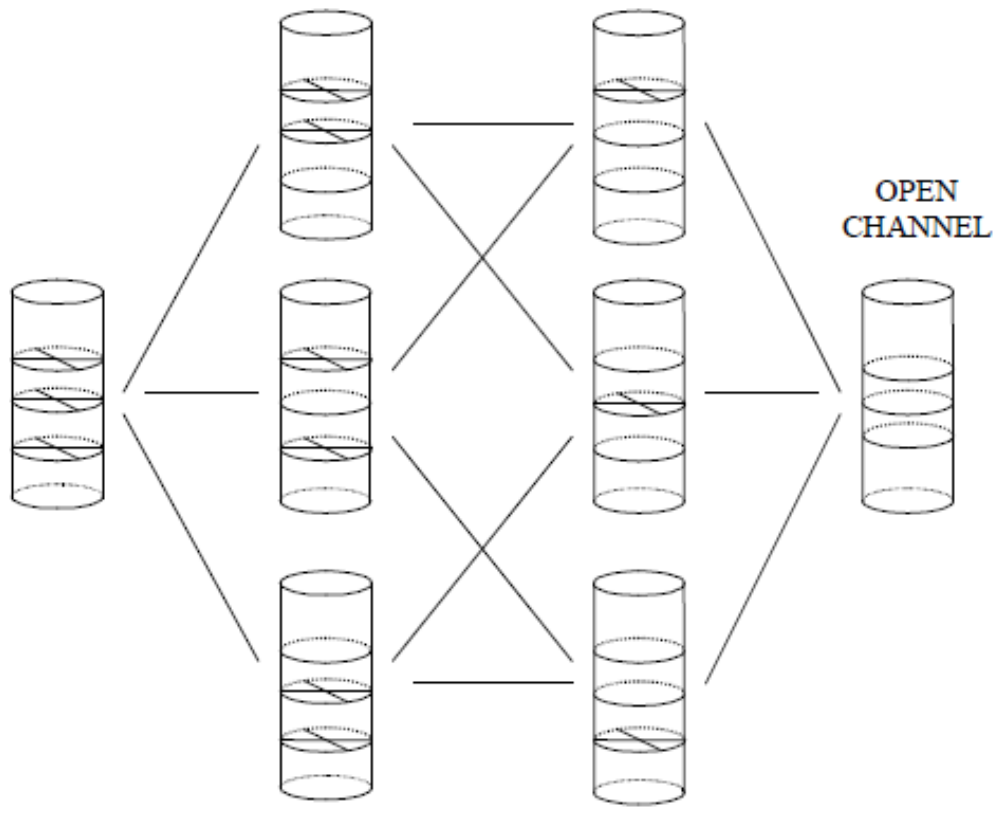
\includegraphics[scale=0.42]{07_1}
    \centering
\end{figure}
The binary activation of a certain channel with \(k\) gates is then defined as
\begin{equation*}
    \xi=\prod_{j=1}^{k}\gamma_{j}
\end{equation*}
where \(\gamma_{j}\) is the binary activation variable for the \(j\)-th gate. Note that
\(\gamma_{j}=1\) if the corresponding \(j\)-th gate is open and, consequently, \(\xi=1\)
only if all the \(k\) gates are open at the same time, otherwise \(\xi=0\).\\
To model the possible \(2^{k}\) states of a channel and the transitions among such states,
a Markov model can be employed. If the states are a finite number (\(2^{k}\)), then also the
transitions are finite.\newpage
Some assumptions are thus necessary:
\begin{itemize}
    \item The states of a single ionic channel are separated by large energy barriers. When the
          channel reaches the right amount of energy, a transition occurs.
    \item The probability to perform a transition depends only on the currently occupied state.
    \item The previous history of occupied channels is not relevant, only the membrane voltage elicits
          a transition, overcoming the energy barrier.
    \item The duration for which the present state remained occupied is not relevant.
\end{itemize}
Henceforth, the time evolution of the probability to occupy state \(S_{i}\) is described by the
equation
\begin{equation*}
    \frac{dP(S_{i},t)}{dt}
    =\sum_{j=1}^{n}P(S_{j},t)P(S_{j}\rightarrow{S_{i}})-\sum_{i=1}^{n}P(S_{i},t)P(S_{i}\rightarrow{S_{j}})
\end{equation*}
where \(P(S_{i},t)\) is the probability of being in state \(S_{i}\) at time \(t\) and
\(P(S_{i}\rightarrow{S_{j}})\) is the probability to have a transition from state \(S_{i}\)
to state \(S_{j}\). Note that, generally speaking, transitions are reversible.\\
If a large number of identical channels is considered, the probability of being in a state \(S_{i}\) can
be reinterpreted as the fraction of channels occupying the \(S_{i}\) state, denoted by \(s_{i}\), while
the transition probability \(P(S_{i}\rightarrow{S_{j}})\) becomes the rate constant of the reaction, \(r_{ij}\).
As a consequence, the previous equation can be rewritten in these terms:
\begin{equation*}
    \frac{ds_{i}}{dt}=\sum_{j=1}^{n}s_{j}r_{ji}-\sum_{i=1}^{n}s_{i}r_{ij}
\end{equation*}
Said so, the HH model should be modified according to the stochastic processes described above:
\begin{gather*}
    C_{m}\frac{dV}{dt}
    =\bar{g}_{Na}\cdot{m^{3}h}\cdot{(V_{m}-E_{Na})}
    +\bar{g}_{K}\cdot{n^{4}}\cdot{(V_{m}-E_{K})}
    +g_{leak}\cdot{(V_{m}-E_{leak})}\\
    \Downarrow\\
    C_{m}\frac{dV}{dt}
    =\bar{g}_{Na}\cdot{m}\cdot{(V_{m}-E_{Na})}
    +\bar{g}_{K}\cdot{n}\cdot{(V_{m}-E_{K})}
    +g_{leak}\cdot{(V_{m}-E_{leak})}
\end{gather*}
where \(m\) and \(n\) are stochastic processes of time and represent the fraction of open channels
selective to Na\({}^{+}\) and K\({}^{+}\) ions respectively.\\
By assuming \(N_{Na,max}\) and \(N_{K,max}\) the total number of sodium and potassium channels
respectively, it can be stated that:
\begin{gather*}
    m=\frac{1}{N_{Na,max}}\sum_{i=1}^{N_{Na,max}}\xi_{Na,i}\\
    n=\frac{1}{N_{K,max}}\sum_{i=1}^{N_{K,max}}\xi_{K,i}
\end{gather*}
Note that the binary activations reported here are to be derived by the binary activation variables,
identifies, described, and modelled through patch-clamp measurements of single channels.\\
An example of a model for potassium channels is shown here, note how the channel has to go through all
the intermediate states in order to reach the open configuration.
\begin{figure}[H]
    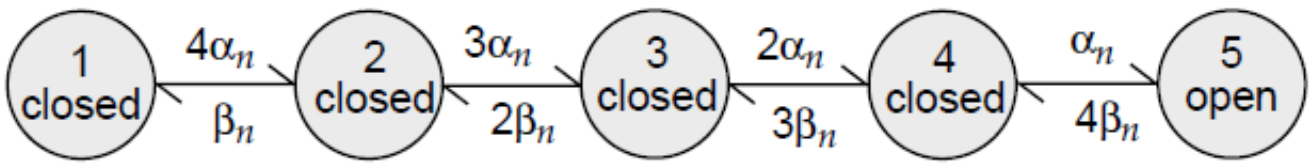
\includegraphics[scale=0.3]{07_2}
    \centering
\end{figure}
Concerning sodium channels, the HH model assumes activation and inactivation processes to be independent,
however that is not the case, as they are interdependent. In particular:
\begin{itemize}
    \item The activation process is voltage-dependent.
    \item The inactivation process is state-dependent (and voltage-independent).
\end{itemize}
Thus, an exaple model for the sodium channels can be the following one:
\begin{figure}[H]
    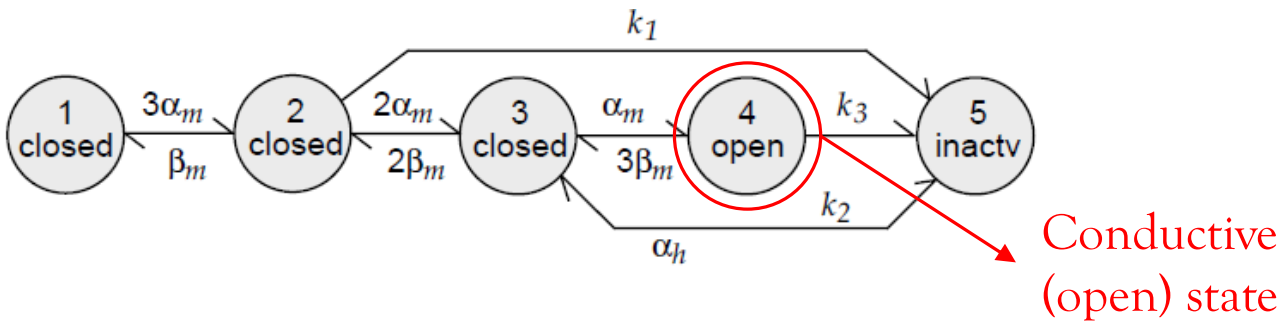
\includegraphics[scale=0.38]{07_3}
    \centering
\end{figure}
The inactive state displayed on the right side means that the channel stops depolarizing, exhibiting
a sort of refractory period, as it is not able to open again and allow the passage of ions.\\
By employing these stochastic models, the behaviour of a single channel is very far from the one
observed through the Hodgkin-Huxley model; nonetheless, by increasing the number of considered
channels the dynamics tend to be coincident with the HH model one. Therefore, it can be said
that stochastic models tends to be equivalent to the HH model as long as a large number of
channels is observed.
\begin{figure}[H]
    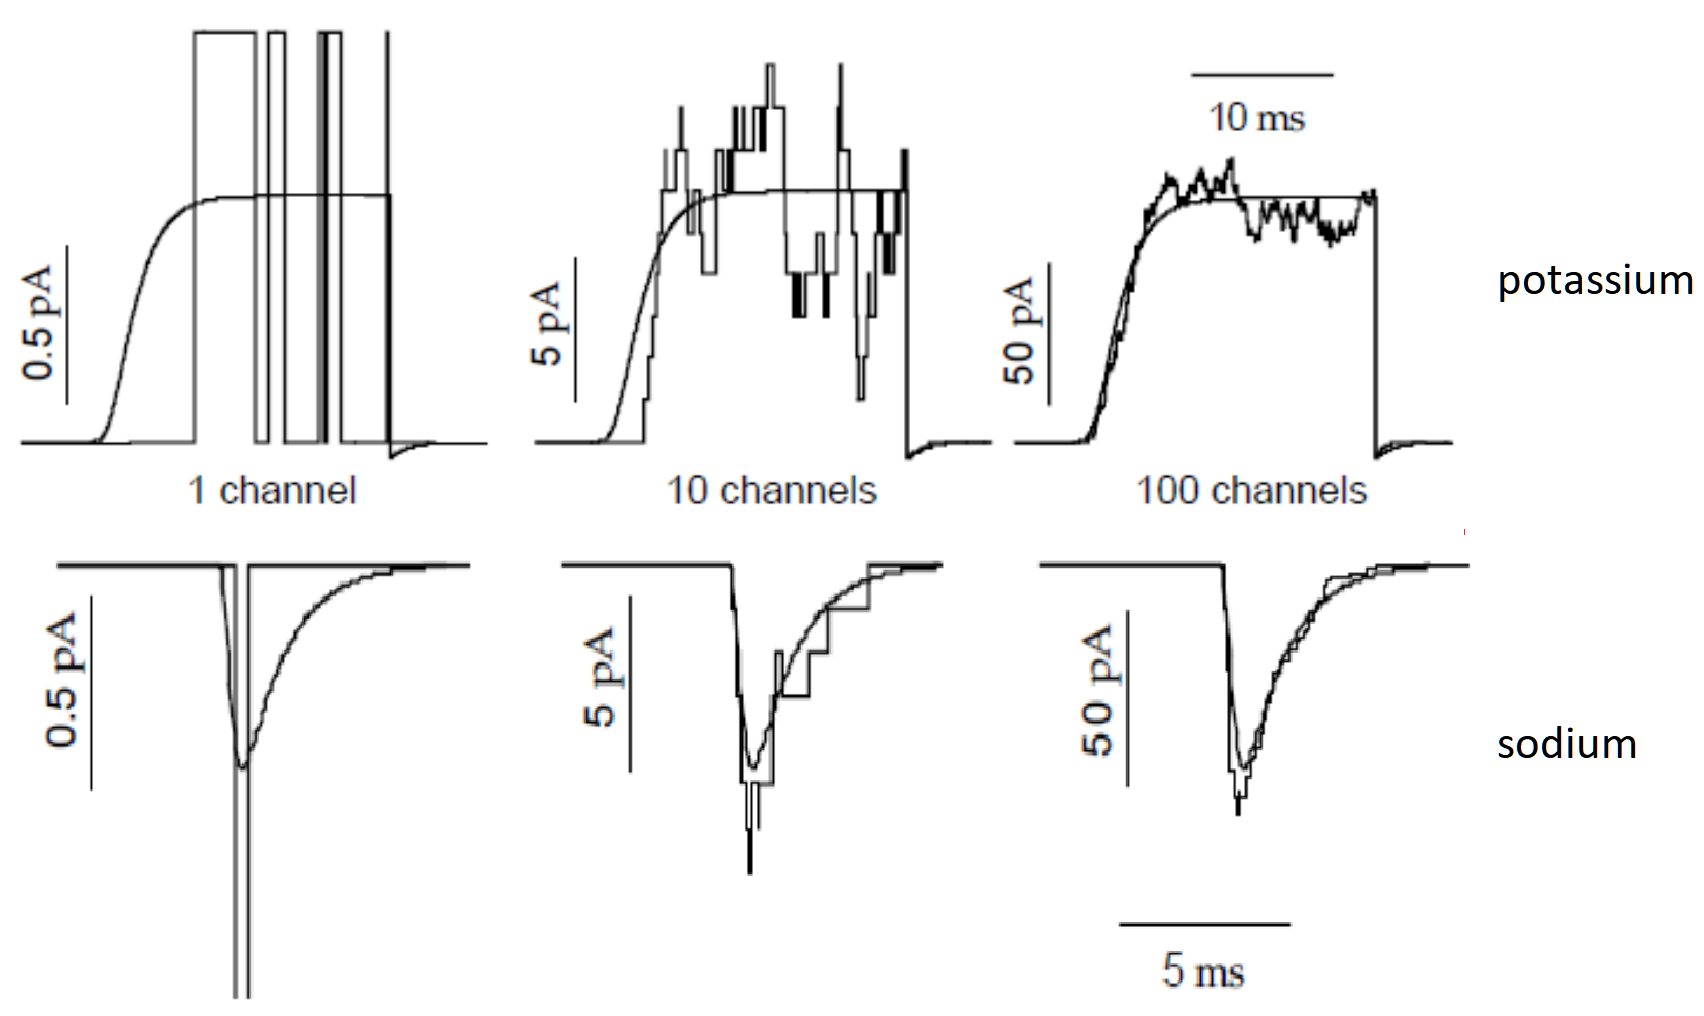
\includegraphics[scale=0.3]{07_4}
    \centering
\end{figure}
\paragraph{Why different models (HH and stochastic ones) display similar behaviours?} This is a
consequence of the speed of the activation process for the Na\({}^{+}\) conductance. In particular,
the activation variable \(m\) of the HH model reaches its voltage-dependent steady-state value
\(m_{\infty}(V_{m})\) extremely rapidly (\(\tau_{m}\approx{1\;ms}\)), making it difficult to distinguish
inactivation processes dependending on \(m\) from those depending on \(V_{m}\).
\begin{figure}[H]
    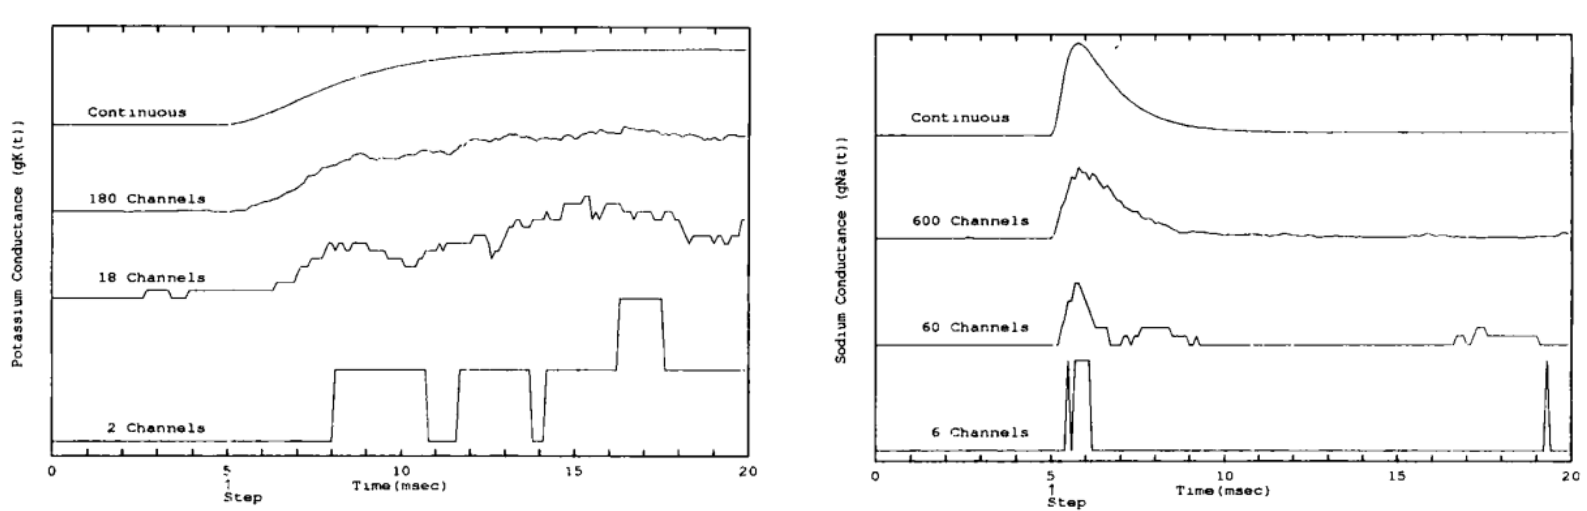
\includegraphics[scale=0.45]{07_5}
    \centering
\end{figure}
Also in the plots above it can be seen that increasing the number of observed channels leads to
a model similar to the HH one. This is true also in the case of current stimulations, as depicted below.
\begin{figure}[H]
    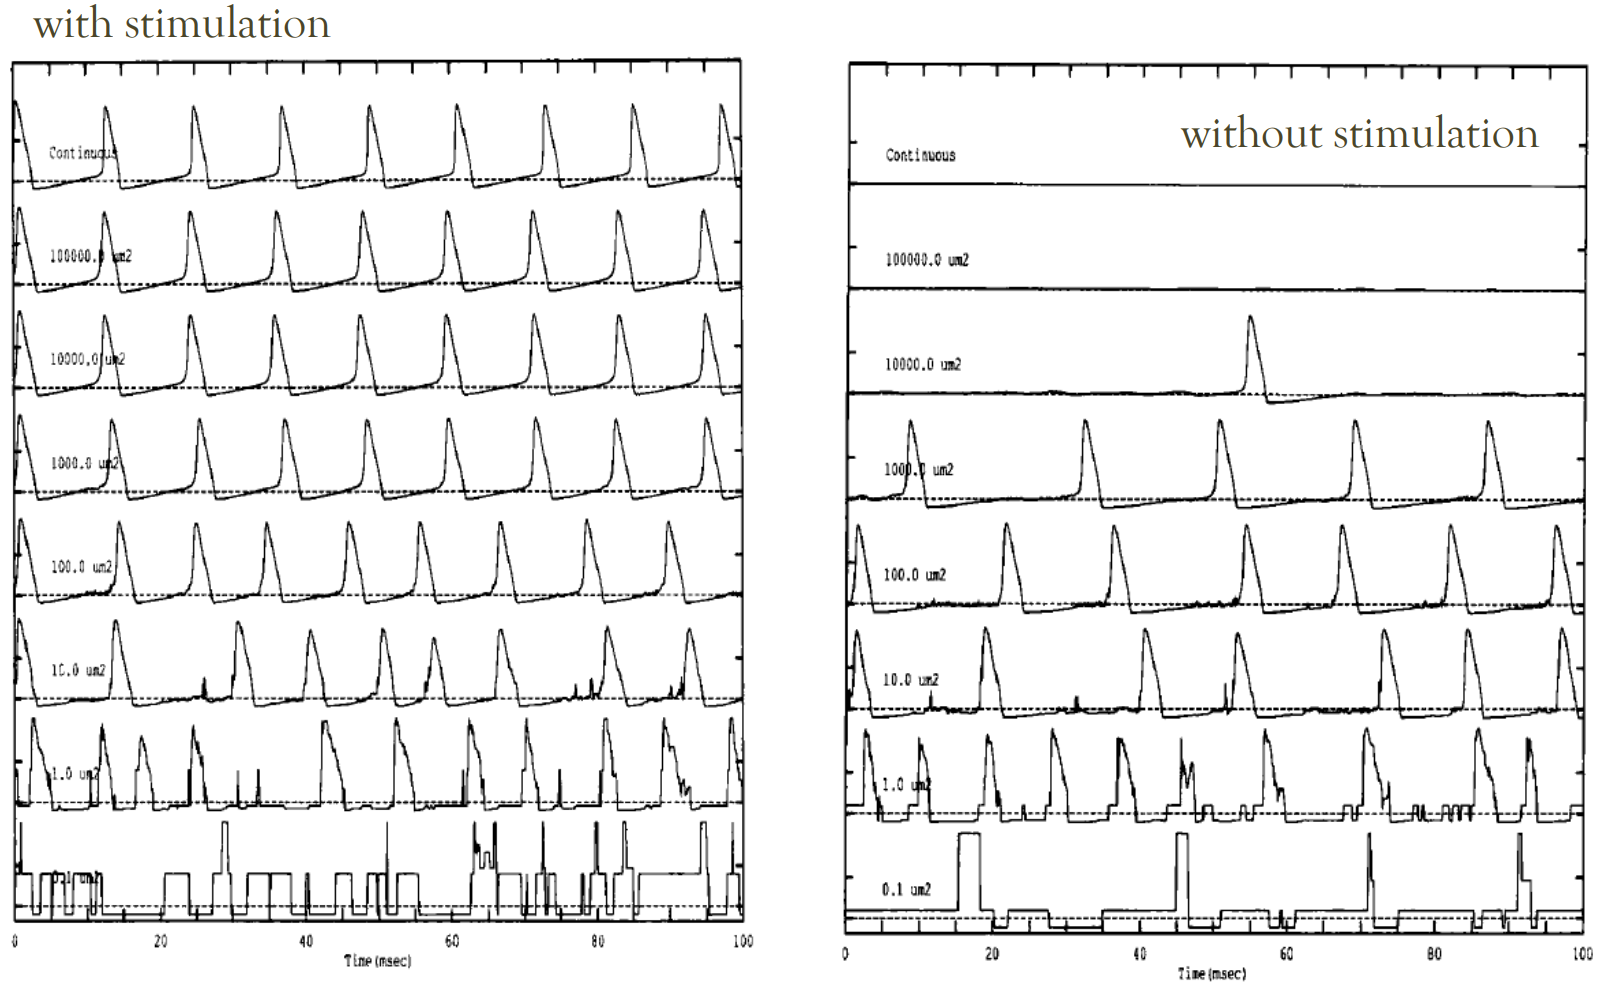
\includegraphics[scale=0.45]{07_6}
    \centering
\end{figure}
Note that the voltage is shown for different amounts of channels as a function of time. With no stimulation,
a flat potential is expected, precisely at the resting potential \(E_{r}\), however if small groups
of channels are considered (a small patch of cell membrane), there are several random fluctuations which
are not able to cancel each other out, resulting in a noisy activity. Similar considerations are true also
in the case where a DC stimulation is present.

\subsection{Voltage-Gated Sodium Channels}
In humans there are nine isomers of voltage-gated sodium channels (VGSC), each one with peculiar kinetics
and tissue distribution. Note that even slight changes of their gating kinetics may cause severe diseases.\\
Ideally, it is deasirable to model these sodium channel isomers through the Markov approach, employing the
possible lowest number of states, as the computational cost should be as light as possible. At the moment,
the model employing the fewest states is the Balbi one, with six states.
\begin{figure}[H]
    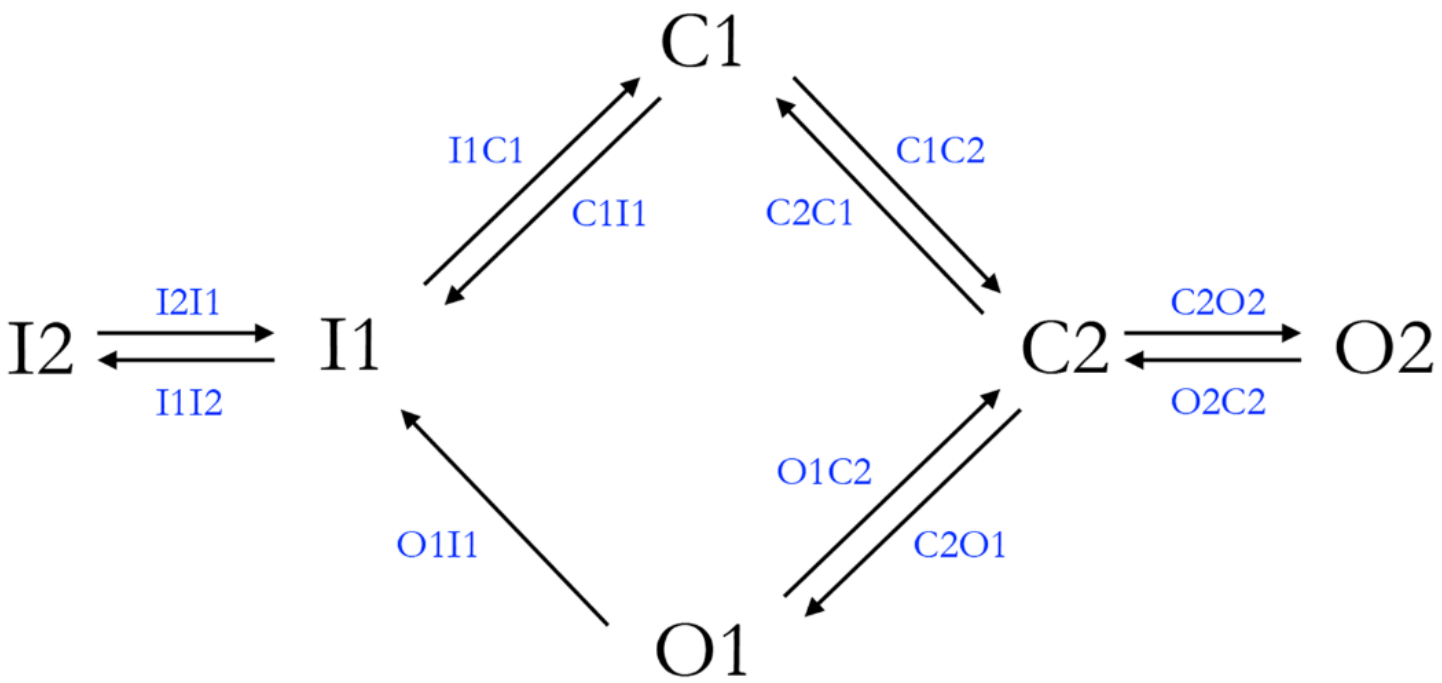
\includegraphics[scale=0.35]{07_7}
    \centering
\end{figure}
The Balbi model is arranged in two closed, two open, and two inactivated states. All transitions are
reversible but one.\\
When developing such a model, one of the most time-consuming and critical steps is the model
parameters tuning, which aims at matching the experimental data.